\chapterimage{Dewatering.jpg} % Chapter heading image

\chapter{Theory - Part I}

\section{Background}
\subsection{Definition of Wastewater}

Wastewater is human polluted water from home and industries. This includes water from:
\begin{itemize}
\item Flushing toilets and urinals  - blackwater.
\item Bathing, showering, and washing clothes and dishes  - greywater.
\item Commercial and industrial activities.
\item ...and often included as wastewater is the storm water which contain pollutants washed off inhabited areas - roads, parking lots, and rooftops.
\end{itemize}

\subsection{Why Treat Wastewater}\index{Why Treat Wastewater}
Although nature has an inherent capability to degrade pollutants, given the quantity of wastewater generated from human activities, centralized wastewater treatment plants are required to treat the wastewater and safely return the treated wastewater back to the environment.  Sewers collect the wastewater from homes, businesses, and industries and deliver it to wastewater treatment facilities before it is released back to the environment through its discharge to a water body like a lake, river or ocean, or land, or reused. 

Wastewater treatment is designed to remove:
\begin{itemize}
\item organic matter
\item inorganic  pollutants including plant nutrients - nitrogen and phosphorous\\
\item pathogenic (disease causing) organisms\\
\end{itemize}

\subsection{Benefits of Treating Wastewater}\index{Benefits of Treating Wastewater}
Wastewater treatment protects:
\begin{itemize}
\item The environment
\item Human health
\end{itemize}

Specifically wastewater treatment allows for the following:

\begin{enumerate}
\item \textbf{Mitigates deterioration of the receiving waters' ecosystem }\\
In the receiving waters, inadequately treated wastewater discharge depletes dissolved oxygen levels due to:

\begin{itemize}

\item Nitrogen and phosphorus are essential for plant growth and are common ingredients in fertilizers. However, nutrient-rich wastewater entering a water body such as a lake or river will promote plant and algae growth which will seriously impact its normal aquatic life including fish through a process similar to the following:

\begin{itemize}
\item Nutrient promote algae bloom
\item Algae bloom prevent sunlight to the native plant spieces below the water's surface causing native plants to die
\item The organic material from the dead plants and algae promote growth of aerobic bacteria which will consume the dissolved oxygen in the water resulting in oxygen depletion.
\item The natural aquatic life including fish, frogs, and turtles will not be able to survive under oxygen depleted conditions and will die or leave that zone.
\end{itemize}
\item Other organic material in present in wastewater, will similarly promote growth of aerobic bacteria intensifying the eutrophication of the receiving waters.
\end{itemize}
\item \textbf{Removal of other harmful pollutants}\\
Organic and inorganic pollutants including metals, such as mercury, lead, cadmium, chromium and arsenic can have acute and chronic toxic effects on aquatic species and wildlife including migratory birds, are removed during the wastewater treatment process.
\item \textbf{Removal of pathogens}\\
Wastewater treatment removes parasites and disease-causing pathogens including bacteria and viruses which allow for:
\begin{itemize}
\item People to continue enjoying recreational activities in the receiving bodies of waters such as lakes and rivers
\item Preventing the contamination of fish and other consumable products obtained from the waters
\item Allow the water body to remain as the source of potable water
\end{itemize}
Thus, treating wastewater prevents \hl{eutrophication} which is the process by which a body of water becomes enriched in dissolved nutrients (such as phosphates) that stimulate the growth of aquatic plant life usually resulting in the depletion of dissolved oxygen resulting in a progressive destruction of its normal aquatic lifeforms.
\item \textbf{Reclaim water for recycle or reuse}\\
Besides protecting human health and the environment, wastewater treatment paves way for establishing the reuse or recycle of treated wastewater.  This benefit is particularly important for densely populated areas with limited access to fresh water supplies.  
\end{enumerate}

\newpage
\section{Wastewater Constituents}
	\subsection{Organics}
		\begin{itemize}
			\item The main reason for treating domestic wastewater is to remove the organic matter.  
			\item Organics are substances containing carbon, hydrogen and oxygen, and some of which may be combined with nitrogen, sulfur or phosphorous.
			\item About 50 percent of the solids present in wastewater are organic.  This fraction is generally of animal or vegetable life, dead animal matter, plant tissue or organisms, and also include synthetic organic compounds.
			\item The principal organic compounds present in domestic wastewater are proteins, carbohydrates and fats together with the products of their decomposition.
			\item Organics are subject to decay or decomposition through the activity of bacteria and other living organisms.  \hl{Since the organic fraction can be driven off at high temperatures, they are also called \textbf{volatile solids}}.\
			\item \emph{Organics in wastewater is typically quantified in terms of oxygen required to oxidize the carbon based material present} in wastewater using the following methods:\\
		\end{itemize}
\subsubsection{Biochemical Oxygen Demand (BOD)}\index{Biochemical Oxygen Demand (BOD)}

			  %     \begin{enumerate}[i.]
			  %     	\definecolor{shadecolor}{RGB}{220,220,220}
					% %%%%%%%%%%%
					% % LEVEL 4 %
					% %%%%%%%%%%%
			  %     	\begin{snugshade*}
			  %     		\item \noindent\textsc{Biochemical Oxygen Demand (BOD)}%@@@@@@@@@@@@@@@@@@%
			  %     	\end{snugshade*}					
			      	\begin{itemize}
			      		\item Oxygen is required for the consumption of organic matter by aerobic bacteria
			      		\item BOD test measures the depletion of oxygen in a wastewater sample over a five day period
			      		\item BOD measures the organic content in terms of oxygen required for the microorganisms to consume the organic material present

			      		\item BOD is typically measured as BOD$_5$ which is the oxygen demand of the wastewater measured after 5 days of the initiation of the test.
			      		\item The test involves incubating a known dilution of wastewater in a 300 ml bottle for 5 days at 20\si{\degree}C.  The dissolved oxygen (DO) content at the start and end of the incubation period is used for calculating the BOD.
			      		\item For the test to be considered valid, the following criteria need to be met: 1) DO consumption during the test must be at least 2 mg/l, 2) DO remaining at the end of the test must be at least 1 mg/l, and 3) DO consumed in blank should be 0.2 mg/l or less
			      		      			
			      		\item BOD is a parameter to measure the strength of wastewater and the measurement of the wastewater treatment plant or treatment process influent and effluent BOD is standard practice to measure its performance.  Typical domestic wastewater BOD is about 200-250 mg/l.
			      		\item The oxygen consumed by the microorganisms during the BOD test is primarily for: 1) Oxidizing the carbonaceous material (cBOD – carbonaceous BOD), and 2) Oxidizing nitrogenous constituents such as ammonia (nBOD – nitrogenous BOD).
			      		\item Thus, BOD (Total) = cBOD + nBOD.  The cBOD and nBOD is measured by adding certain chemical inhibitors which will inhibit the bacteria responsible for consuming the nitrogenous matter, thus measuring only the cBOD as part of the BOD test.
			      		\item Since not all of the organics is metabolized in the 5 days of the regular BOD test, certain wastewater discharge permits require reporting of the ultimate BOD value (BOD$_U$)\\
			      	\end{itemize}

			    \subsubsection{Chemical Oxygen Demand (COD)}\index{Chemical Oxygen Demand (COD)}
			      	% \begin{snugshade*}
			      	% 	\item \noindent\textsc{Chemical Oxygen Demand (COD)}%@@@@@@@@@@@@@@@@@@%
			      	% \end{snugshade*}		  
			      	\begin{itemize}
			      		\item The COD test involves using chemical oxidizers to measure the oxygen demand of the wastewater.
			      		\item As the chemical oxidizers will oxidize other constituents present, including inorganic matter, the COD value of wastewater will be higher than the BOD.  
			      		\item The COD test can be conducted rather quickly than the 5 day BOD test, it is an effective method to quantify the wastewater strength and process efficiencies and allow operators to make timely process adjustments.
			      	\end{itemize}


		
			\hl{BOD measures the amount of oxygen required by the microorganisms present to consume the organic material while COD measures the chemical oxidation required to oxidize all chemicals including organics present in wastewater.  BOD value of typical domestic sewage is about 200 - 250 mg/l while the COD value ranges from 300 - 450 mg/l.  Typical BOD:COD ratio ranges from 0.5-0.8.}\\


\subsection{Solids}\index{Solids}
% 		\pagebreak
% 				\begin{snugshade*}
% 			\item \noindent\textsc{Solids}
% 		\end{snugshade*}	
		Like BOD, wastewater solids is another critical parameter for establishing the wastewater strength and determining treatment process efficiencies. 
		\begin{itemize}
			\item The \texthl{solids can be classified as suspended or dissolved} based upon its ability to pass through a standardized filter paper.
			\item When the wastewater is filtered:
			      \begin{itemize}
			      	\item the residual solids remaining on the filter paper after drying in an oven at 103\si{\degree}C is the \hl{suspended solids} portion, and 
			      	\item the solids remaining after drying the filtrate are the \hl{dissolved solids}.
			      \end{itemize}
			\item Suspended solids include larger floating particles and consist of sand, grit, clay, fecal matter, paper, pieces of wood, particles of food and garbage, and similar materials.
			\item Suspended solids can be categorized based upon its settling characteristics as:
			      \begin{itemize}
			      	\item \hl{Settleable}
			      	\item \hl{Non-settleable}
			      	      \begin{itemize}
			      	      	\item \hl{Colloidial}-small, charged (typically negative) particles which do not settle easily.  Some of the colloidial particles are small enough to pass through the filter paper used for filtering the suspended solids
			      	      	\item \hl{Floatable}-example oil and grease and small plastics
			      	      \end{itemize}
			      \end{itemize}
			\item Dissolved solids in wastewater include organics.  However, the major elements of dissolved solids are inorganic ions such as Ca$^{+2}$, Mg$^{+2}$, Cl$^-$, SO$_4$ $^{-2}$ , HCO$_3$ $^-$, Fe$^{+2}$, PO$_4$ $^{-3}$, NO$_3$ $^-$.  These ions are part of the dissolved salts such as sodium chloride (NaCl), calcium bicarbonate (Ca(HCO$_3$)$_2$), magnesium phosphate (Mg$_3$PO$_4$) and others which are normally present in water and wastewater. 
			      \begin{itemize}
			      	\item Conductivity or electrical conductance (EC) measurement is typically conducted as the wastewater enters the plant as \hl{conductivity provides an indirect and simple measure of the amount of dissolved solids present.}  
			      	\item Conductivity or electrical conductance (EC) is a measure the amount of electrical current that can be conducted by a solution.  
			      	\item The conductance of electricity in a solution is due to the presence of dissolved inorganic ions 
			      	\item The higher the concentration of these ions, the higher is the conductivity. 
			      	\item \underline{Conductivity is measured in the units of mhos/cm or Siemens/cm.}  (Note:  mhos is the reverse of ohm which is a measure of resistance).
			      	\item Typical wastewater conductivities range from 50 to 1500 S/cm
			      \end{itemize}
			\item Both suspended and dissolved solids can be either \hl{volatile (organic)} or \hl{fixed (inorganic)}.
			\item \hl{Total Solids is thus a sum of TSS and dissolved solids or volatile and fixed solids.}
			      \begin{itemize}
			      	\item The volatile solids are typically of plant or animal origin .
			      	\item The fixed solids include sand, gravel and silt as well as the dissolved salts.
			      \end{itemize}
			      \begin{minipage}{0.5\textwidth}
			      	\item The volatile or fixed fractions are quantified by incinerating the solids in a muffler furnace at 550\si{\degree} which removes only the volatile solids leaving only the fixed solids behind.
			      	\item In terms of the size of the solids, the distribution is approximately thirty percent suspended and about seventy percent dissolved solids - which includes the colloidal particles which have passed through the filter paper.\\ 
			      	\item As primary treatment process involve settling of solids, establishing the settleable portion of the suspended solids is important.\\  
			      	\item \hl{The settleable solids are quantified using an Imhoff cone and are reported in ml/L}.  Imhoff cone is a 1 liter, clear cone shaped container, with volume graduations (ml) at the bottom.
			      						
			      \end{minipage}	
			      \begin{minipage}{0.5\textwidth}
			      	\begin{center}
			      		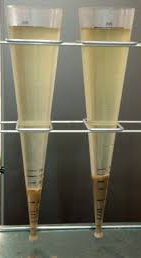
\includegraphics[scale=0.7]{ImhoffCone}\\
			      		Imhoff Cone\\
			      		\textit{Note the ml markings at the bottom of the cone}
			      		
			      		
			      	\end{center}
		      \end{minipage}
%			      \end{minipage}
			      	\item One factor which affects settleability is the conveyance time of the sewage to the treatment plant. 			
			      	\item The settleable component of the suspended solids will decrease as the sewage becomes more septic due to longer conveyance times.
			\item Influent and effluent total suspended solids are measured to establish the overall treatment and individual process efficiencies.  
			\item Volatile solids measurements before and after biological processes such as secondary treatment and digestion provide information on the process efficiency.\\
		\end{itemize}

% 			\end{enumerate}
	\subsubsection{Summary of Wastewater Solids}\index{Summary of Wastewater Solids}		
% 			\begin{snugshade*}
% 				\item \noindent\textsc{Summary of Wastewater Solids}
% 			\end{snugshade*}
			\begin{itemize}
				\item Solids in wastewater can be categorized as dissolved or suspended
				      \begin{itemize}
				      	\item Suspended solids can be further categorized as settleable or unsettleable
				      \end{itemize}
				\item Solids can also be categorized as organic (aka: volatile) or inorganic (aka: fixed)
				\item Colloidial particles are small sized particles some of which pass through the filter and accounted as part of dissolved solids
				\item TSS - Total Suspended Solids are the solids that are captured on the filter paper upon filtration of the wastewater sample.  
				\item Wastewater samples typically analyzed for TSS include:  plant, primary and secondary processes - influent and effluent.  TSS is reported in mg/l
				\item TS - Total Solids are solids content of sludge.  TS of sludge is established by drying a preweighed quantity of sludge in an oven and is typically reported as \% solids - which is how many parts (by weight) of solids per 100 parts (by weight) of sludge.
				\item Volatile solids are solids that are removed when the solids are incinerated at 550C.  The solids that remain after incineration are fixed or non-volatile or inorganic solids.
			\end{itemize}
	\subsubsection{Wastewater Solids Content}\index{Wastewater Solids Content}			
% 			\begin{snugshade*}
% 				\item \noindent\textsc{Typical influent wastewater contains:}
% 			\end{snugshade*}
			\begin{itemize}
				\item Less than 0.1\% total solids.  Total solids concentration in typical wastewater is about 750mg/l
				\item The total solids are 50\% organic (volatile) and 50\% inorganic (fixed)
				\item Of the total solids, dissolved solids constitute about 70\% of the solids and the remaining 30\% solids are suspended solids
				\item 40\% of the dissolved solids are volatile the remaining 60\% are fixed
				\item 70\% of the suspended solids are volatile and the remaining 30\% are fixed
			\end{itemize}
			% \clearpage\thispagestyle{empty}
			\begin{figure}[!htbp]
			\vspace{2cm}
				\begin{center}
					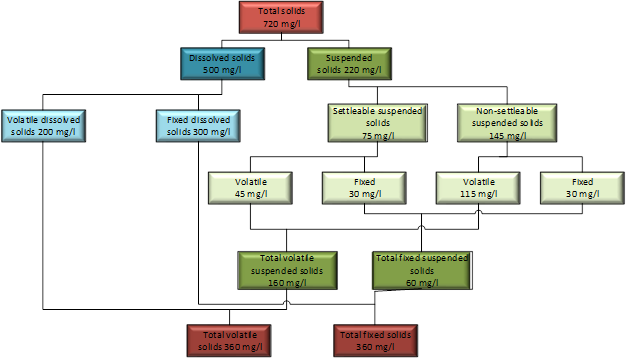
\includegraphics[scale=0.8]{WastewaterSolids}\\
					\caption{Typical Wastewater Solids Concentrations}
				\end{center}
				\end{figure}
% % 			\end{enumerate}
				
\subsection{Nutrients}\index{Nutrients}	
% 			\begin{snugshade*}
% 				\item \noindent\textsc{Nutrients}
% 			\end{snugshade*}	
			\begin{itemize}
				\item Plant nutrients - nitrogen and phosphorous, present in wastewater effluent discharge, promote growth of plant and algal matter in the receiving waters causing destruction of the normal aquatic life mainly due to oxygen depletion - eutrophication.
				      
				\item Because of the potential impacts of the presence of these nutrients in wastewater effluent on the receiving waters,  limits on the levels of these nutrients is typically stipulated in the treatment plant's wastewater discharge permit.
				      
				\item Typically, conventional secondary treatment processes are designed primarily remove the organics from the wastewater.  Secondary treatment process designed to additionally remove nutrients is deemed as tertiary or advanced treatment is termed as Biological Nutrient Removal (BNR).
			\end{itemize}
	\subsubsection{Nitrogen}\index{Nitrogen}				
% 			\begin{enumerate}%@@@@@@@@@@@@@@@@@@%
% 				\definecolor{shadecolor}{RGB}{220,220,220}
% 				\begin{snugshade*}
% 					\item \noindent\textsc{Nitrogen}%@@@@@@@@@@@@@@@@@@%
% 				\end{snugshade*}

	\textbf{Forms of nitrogen:}\\	
% 				\begin{itemize}
% 					\item Forms of nitrogen:\\
					      \begin{itemize}
					      	\item About 60\% of nitrogen in wastewater is present as ammonia nitrogen (about 60\%).  The ammonium nitrogen is present either in the form of ammonia (NH$_3$ ) or as ammonium (NH$_4^+$ ) ion.   These two forms can rapidly change from one to the other depending on pH and temperature.  Under low pH (acidic) or neutral conditions – pH less than or equal to 7, ammonia exists mostly as ammonium.  Ammonia becomes the dominant form as the pH increases to 8 and beyond.
					      	\item The other dominant form of nitrogen, about 40\% of the total nitrogen is as organic nitrogen
					      	\item Nitrogen measured as Total Kjeldahl Nitrogen (TKN) which is the sum of the organic nitrogen and the ammonia nitrogen concentrations.  Total inorganic nitrogen is the total concentration of ammonia nitrogen, NO3-, and NO2-.   Table provides the concentrations and forms of nitrogen in wastewater.
					      \end{itemize}
					      \setlength{\arrayrulewidth}{0.7mm}
					      \setlength{\tabcolsep}{8 pt}
					      \renewcommand{\arraystretch}{0.8}
					      \begin{center}
					      \begin{figure}[!htbp]
					      	\noindent \begin{tabular}[!htbp]{ |p{6cm}|p{2.0cm}|p{2.5cm}|p{2.cm}|}
					      	\hline
					      	\multicolumn{4}{|c|}{\textbf{Forms of Nitrogen in Wastewater}} \\
					      	\hline
					      	%\thead{A Head} & \thead{A Second \\ Head} & \thead{A Third \\ Head} \\
					      	%\hline%
					      	
					      	\hspace{1.8 cm}Forms of Nitrogen & \hspace{0.25 cm} Formula & \hspace{.4 cm} Found in & \hspace{.4 cm} Typical \newline \hspace{.2 cm}Concentration\\
					      	\hline
					      	\small Ammonia/Ammonium & \small NH$_3$/NH$_4^{\enspace +}$ &  \small Influent wastewater & 30-50 mg/l\\
					      	
					      	Total Kjeldahl Nitrogen \newline  \small (Ammonia/Ammonium + Organic Nitrogen) &  \small TKN &  \small Wastewater \newline  \small effluent  & 30-60 mg/l \\
					      	
					      	\small Total Inorganic Nitrogen \newline  \small (Ammonia/Ammonium + Nitrite + Nitrate) & \small TIN &  \small  Wastewater \newline  \small effluent  & 1-40 mg/l \\
					      	
					      	\small Nitrate  & $NO_3^{\enspace -}$ &  \small Nitrified effluent &  \small 1-35 mg/l \\
					      	
					      	\small Nitrate  &  $NO_2^{\enspace -}$ &  \small Partially nitrified effluent &  \small 0.1-2 mg/l \\
					      	
					      	\hline
					      	\end{tabular}
					      	\caption{Forms of Nitrogen}
					      	\end{figure}
					      \end{center}
					      
		\subsubsection{Phosphorous}\index{Phosphorous}			
		\textbf{Forms of phosphorous:}\\
					      \begin{itemize}
					      	\item The principal forms are organically bound phosphorus, polyphosphates, and orthophosphates.
					      	\item Organically bound phosphorus originates from body and food waste and, upon biological decomposition of these solids, is converted to orthophosphates. 
					      	\item Polyphosphates originate from synthetic detergents and are hydrolyzed to orthophosphates. Thus, the principal form of phosphorus in wastewater is assumed to be orthophosphates, although the other forms may exist. Orthophosphates consist of the negative ions PO$_4$$^{3-}$, HPO$_4$$^{2-}$, and H$_2$PO$_4$ $^-$.  These may form chemical combinations with cations (positively charged ions).
					      \end{itemize}

\subsubsection{Oil and Grease}\index{Oil and Grease}	
			Fats, oil and grease in wastewater originate from homes, food establishments and industries.
			\begin{itemize}
				\item Oil and grease content of wastewater is established in the laboratory by extracting it with a solvent - \textit{n}-hexane.  The concentration of oil and grease is reported in mg/l and typical oil and grease content of wastewater ranges from 80 - 120 mg/l
				\item Presence of excessive oils and grease could potentially impact the secondary treatment process
				\item Oils and grease are removed as floatables in primary treatment and sent with the sludge to the digesters
			\end{itemize}
\newpage	
\section{Wastewater Sampling}		
		\begin{itemize}
			\item Field or laboratory measurement of a certain parameter is critical in wastewater treatment operations to obtain information about wastewater characteristics in order to either characterize a wastewater stream, or to monitor a treatment process or for permit compliance.  
			\item A sample is a small part of the whole representing the whole.  Thus, a sample needs to be such that it truly represents the entire population – which in a wastewater operations could be either a wastewater stream, wastewater solids or a chemical used.
		\end{itemize}
		
\subsection{Sampling Methods}\index{Sampling Methods}
\subsubsection{Grab Samples}\index{Grab Samples}
				\begin{itemize}
					\item A grab sample is a sample collected at a specific spot at a site over a short period of time.  
					\item Grab sampling allows for instantaneous analysis of parameters such as pH, dissolved oxygen, chlorine residual, temperature and other parameters which change rapidly with time.
					\item A grab sample represents a snapshot of space and time of a process stream.
					\end{itemize}
\subsubsection{Composite Samples}\index{Composite Samples}
				\begin{itemize}
					\item A composite sample is a collection of discrete samples are combined over a certain period or space and therefore represent the average performance of a wastewater treatment plant or a process during the collection period.\\  
					\item Composite sampling can be either based on:
					      
					      1. constant time interval (time proportioned sampling)\\
					      2. constant wastewater volume interval (flow-proportioned sampling), and\\
					      3. treatment process space - includes samples taken at different depths\\
					      
					\item Composite samples are typically collected using automated samplers which can be programmed to collect samples at pre-established time intervals – for time proportional sampling.
					\item Time and space composite samples are collected by adding equal volumes of samples collected from different times or locations.  
					\item Flow proportional composite samples comprise of volume of each subsample based on flow.\\  
				\end{itemize}
				
			\begin{center}
				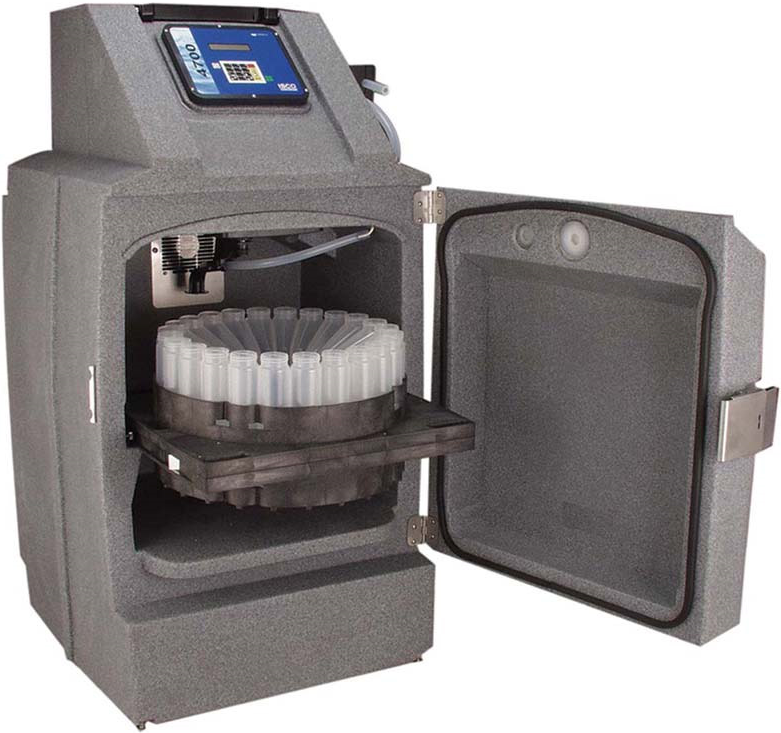
\includegraphics[scale=0.2]{Autosampler} \hspace{2cm} 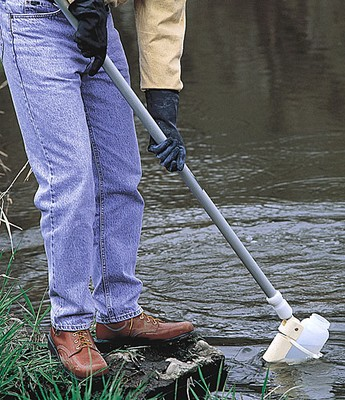
\includegraphics[scale=0.37]{Grabsampler}\\
			\end{center}
			\hspace{2.3cm} Automated Sampler \hspace{2.0cm} \parbox{\textwidth}{Grab Sampling Using a Long Handle Dipper}\\

\subsubsection{Sampling Precautions and Protocols}\index{Sampling Precautions and Protocols}
			\begin{itemize}
				\item Samples should represent the major portion of the process or the process stream and should be taken from places where the mixing is thorough, avoiding dead spots and areas of heavier or lighter loadings. 
				\item The collected sample is invariably exposed to conditions very different from the original source and is subject to change due to chemical and microbiological activity.  
				\item Thus, in order to ensure integrity of sample, sample preservation techniques specific to the analysis to be performed is needed.  
				      \begin{itemize}
				      	\item The preservation technique should not only allow for stabilizing the parameter to be analyzed, it should also not interfere with the analyses.  
				      	\item The common preservation techniques involve use of proper containers, temperature control, addition of chemical preservatives, and observance of the recommended maximum sample holding time.
				      \end{itemize}
			\end{itemize}
			
\subsubsection{Bacteriological Sampling}\index{Bacteriological Sampling}
\begin{itemize}
\item Always collected as a grab
\item A clean, sterile borosilicate glass or plastic bottle containing sodium thiosulfate is used. Sodium thiosulfate is added to remove residual chlorine which will kill coliforms during transit. If the sample is not preserved or maintained under proper conditions until the test is conducted in the laboratory, the test would provide erroneous results
\item Samples must be refrigerated if they cannot be analyzed within 1 hour of collection
\item Samples must be handled with care to prevent contamination and adverse conditions such as prolonged exposure to direct sunlight
\item Maximum holding time for state or federal permit reporting purposes is 6 hours
\end{itemize} 

\subsection{Data Reporting}\index{Data Reporting}	
		\begin{itemize}
			\item Arithmetic mean is typically calculated for reporting data where multiple samples have been collected and analyzed for the same process stream at different times and for reporting average value over a certain time period – daily, monthly etc.\\ \item Arithmetic mean mathematically is calculated by adding all the result values and dividing by the total number of data points.\\
		\end{itemize}
		Mathematically the arithmetic mean is represented as:\\
		$$\bar{x}=\frac{\sum_{i=1}^{n} x^i}{n} = \frac{x_1+x_2+x_3...x_n}{n}$$
		For example:\\
		Arithmetic mean of the following set of data points:  200, 304, 250, 400 is calculated as:\\
		\vspace{10pt}
		Arithmetic Mean = $\frac{200 + 302 + 250 + 400}{4}= 288$\\
		\vspace{10pt}
		For data sets for analysis such as fecal coliform could include values which vary by several orders of magnitudes, using the arithmetic mean to report the average value is not appropriate as the lower or higher values would bias the calculated mean.\\
		\vspace{10pt}
		For example, consider a data set with values:  260, 300, 500, 5,000, 320 and 200.\\
		\vspace{10pt}
		The arithmetic mean = $\frac{260+300+500+5,000+320+200}{6} = 3,444$\\
		Here the 5000 value completely skews the arithmetic mean.
		
		Therefore, for such tests, the geometric mean calculation is used for reporting the average value.\\
		
		
		Mathematically a geometric mean is represented as:\\
		$$\Bigg(\prod_{i=a}^n\Bigg)^{\frac{1}{n}}=\sqrt[n]{a_1*a_2*a_3...a_n}$$
		 
		Calculation method:\\
		1.	Find the product of all the data points (analogous to first calculating the sum of all the data points when calculating the arithmetic mean)\\
		260*300*500*5,000*320*200 = 12,480,000,000,000,000\\
		2.	Raise the product to the inverse of the number of data points\\
		(*Using the power function of a scientific calculator)\\
		Here n (\# data points) = 6 $\implies$ geometric mean = $(12,480,000,000,000,000)^{\frac{1}{6}}   = 482$

\newpage
\section{Collection}\index{Collection}	
The collection system resembles a tree that branches out from the treatment plant to collect the wastewater from individual sources.

\subsection{Wastewater Collection Piping}\index{Wastewater Collection Piping}	
	\begin{itemize}
		\item A \hl{lateral} is the piping that connects the public sewer to the building. 
		\item Laterals flow into larger lines called \hl{mains}.
		\item Mains carry the flow into the largest lines in the system, called \hl{trunk lines}. 
		\item A trunk line is the pipe that brings water into the treatment plant.
	\end{itemize}
\subsection{Sanitary Sewer Systems}\index{Sanitary Sewer Systems}

Sanitary sewer systems collect and convey wastewater from residential, commercial and industrial sources to a centralized wastewater treatment facility for treatment. 

\subsubsection{Storm-water systems}\index{Storm-water systems}

Storm-water systems are designed solely for the conveyance of storm-waters waters directly to streams, rivers, lakes, or the ocean.
 
\subsubsection{Combined sewer systems}\index{Combined sewer systems}
\begin{itemize}
\item Combined sewer systems collect and convey sanitary sewage and urban runoff in a common piping system.
\item Combined sewers could potentially cause serious water pollution problems during combined sewer overflow (CSO) events when wet weather flows exceed the sewage treatment plant capacity.
	\end{itemize}
\begin{center}
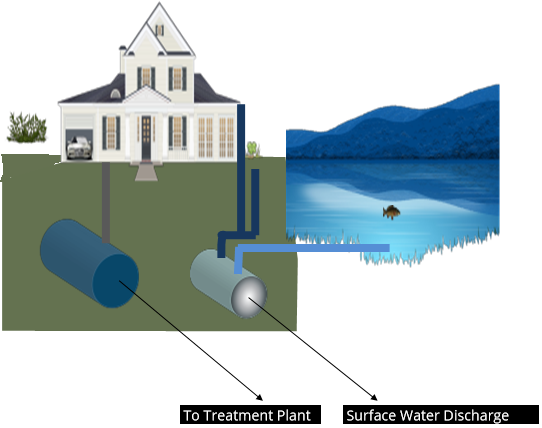
\includegraphics[scale=0.45]{SeperatedSystem1} \hspace{1 cm} 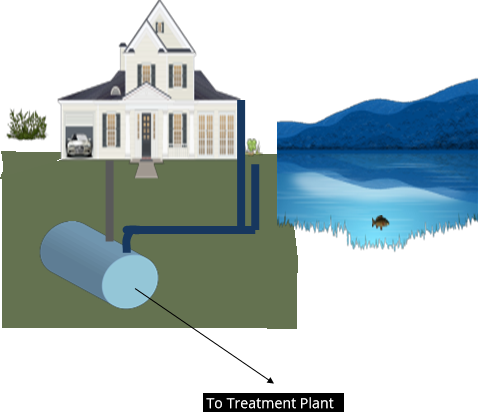
\includegraphics[scale=0.45]{CombinedSystem1}
\end{center}
			\hspace{2.6cm} Separated System \hspace{3.2cm} \parbox{\textwidth}{Combined System}\\

\subsection{Collections Systems Basics}\index{Collections Systems Basics}
	\begin{itemize}
\item The primary type of a collection system is a \hl{gravity system}. A gravity system is so named because the wastewater flows down gradient in the sewer, driven by forces of gravity. 
\item The collection system includes the gravity sewers, force mains, manholes, pumping equipment, and other facilities that collect and convey the water to a wastewater treatment plant. 
\item Sewers are generally laid at a minimum slope to ensure open channel flow through the pipe at a \hl{minimum velocity of 2.0 feet per second}. The minimum velocity is required to ensure that solids do not settle out in the sewer.  
\item When the sewer lines reach a certain depth, the flow must be lifted back through a lift or pump station.  
\item \hl{Lift stations} are built whenever wastewater must be pumped to a higher altitude, whether it's to lift water up so that it can gravity flow or to pump it over a rise or hill.  
\item The discharge from the pump station may be to another gravity sewer at that location or through a pressurized force main. 
\item Key elements of lift stations include a wastewater receiving well (wet-well), pumps and piping with associated valves.
\item The size of the wet well affects the operating of the station. If a wet well is too small, excessive starting and stopping of the pump motors will occur, resulting in premature failure. If the wet well is too large, solids will tend to settle on the bottom, blocking the pump suction line and leading to the generation of hydrogen sulfide and methane.
\item The dry well is the portion of the dry well/wet well pumping station that houses the necessary equipment required to pump the wastewater. The dry well is so named because it is isolated from the incoming wastewater.
\item Centrifugal pumps are the most common type of pump found in wastewater pumping stations. 
\item In the USA, wastewater generated in a typical home is about 70 gal/day/person
\end{itemize}

\newpage
\section{Preliminary Treatment}\index{Preliminary Treatment}

			\begin{itemize}
				\item The objective of preliminary treatment is to remove coarse solids and other large materials often found in raw wastewater
				\item Removal of these materials is necessary to enhance the operation and maintenance of subsequent treatment units\\
				\item Preliminary treatment operations typically include a combination of the following processes:
					\begin{itemize}
						\item Screening
						\item Grinding or shredding
						\item Flow measurement
						\item Grit removal
						\item Pre-aeration
						\item Flow equalization
					\end{itemize}
			\end{itemize}

				
		\subsection{Process Elements of Preliminary Treatment}\index{Process Elements of Preliminary Treatment}	
			
		\subsubsection{Screening}\index{Screening}
					\begin{itemize}
						\item Screening is typically the first unit in a preliminary treatment
						\item Screening allows for the capture of coarse solids as pieces of cloths garbage so as to protect pumps and other units from clogging. 
						\item Screens may consist of vertical or inclined bars (bar racks or bar screens), wire mesh or perforated plates having either circular or rectangular openings. 
						\item Screens remove the large, entrained, suspended or floating solids such as pieces of wood, cloth, paper, plastics, garbage, etc.
						\item Debris collected on the screen can be cleaned manually or automatically using chain driven rakes 
						\item The retained material at screens - screenings, is collected and hauled to landfill for disposal
						\item The quantity of screenings removed varies by location and is a function of the clear opening of the screen.
						\item Barmuinitors combine the function of a screen and a grinder.  The ground material is returned to the wastewater flow for removal during primary treatment.
					\end{itemize}

\begin{figure}
\begin{center}
    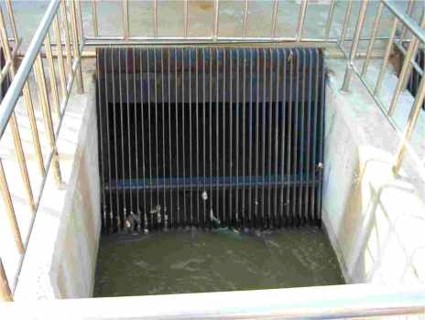
\includegraphics[width=0.7\linewidth]{Barscreen}\\

Barscreen - No rakes
\end{center}
  \end{figure}
  

		\subsubsection{Grinding and Shredding}\index{Grinding and Shredding}

					\begin{itemize}
\begin{minipage}{\textwidth}	\item Comminutor(Grinder) consist of fixed, rotating or oscillating teeth or blades, acting together to reduce the solids to a size which will pass through fixed or rotating screens grind rags into small chunks
\item The comminutors are installed in wastewater channel and they grind the larger solids without actually removing them from the wastewater.  These devices may be installed before the screens or as a combination of screen and cutters (barmunitors).
					\end{minipage}	
					\end{itemize}
					\begin{minipage}{\textwidth}
					\begin{center}
      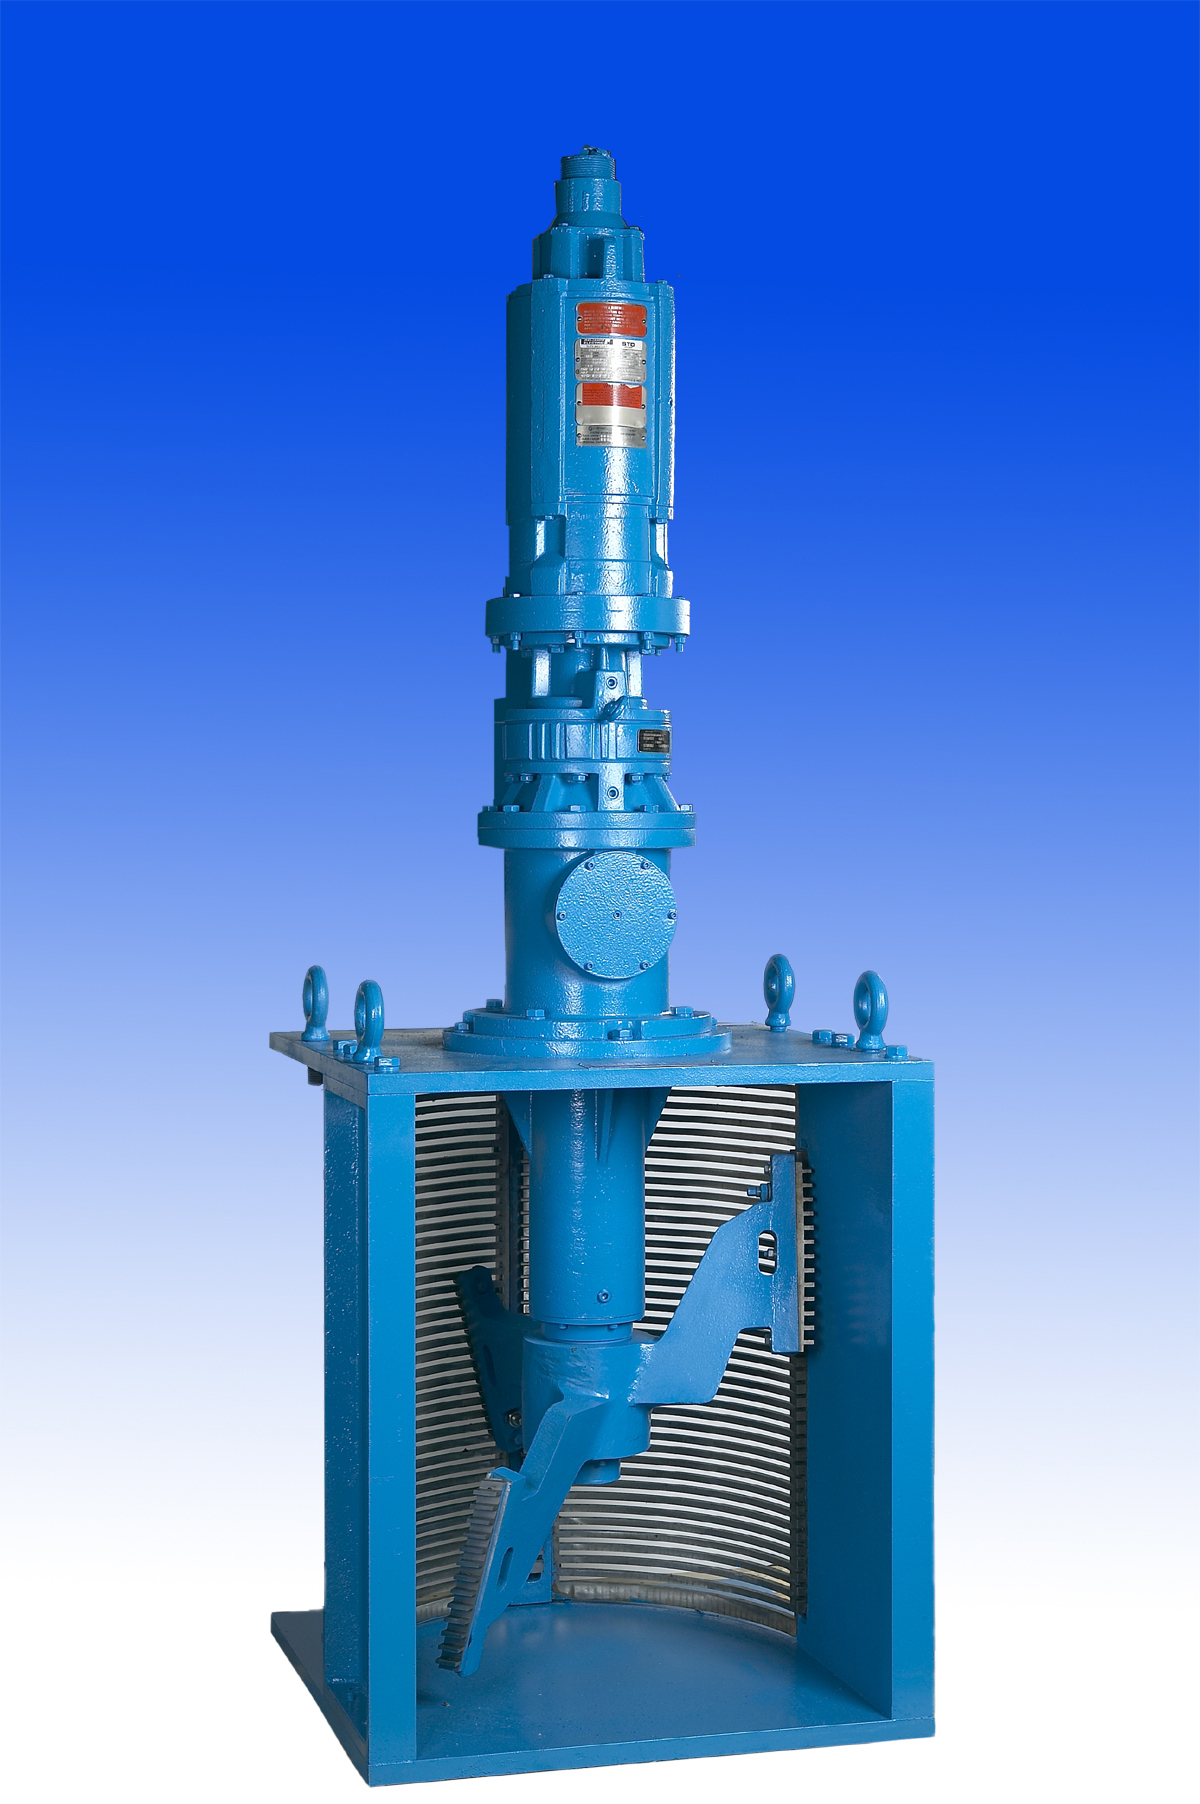
\includegraphics[width=0.3\linewidth, height=70mm]{Comminutor}\\
      Comminutor\\
\end{center}
    \end{minipage}
  
		\subsubsection{Flow Measurement}\index{Flow Measurement}
					\begin{itemize}
						\item Wastewater flow to a treatment plant is not constant but varies in a diurnal (daily) pattern reflecting domestic water use activity.
						\item Continuous flow measurement is necessary in order to monitor diurnal variations in flow which may affect treatment plant efficiency.\\
						\item Devices used for flow measurement as part of the preliminary treatment can be placed in a channel or in a pipe.
					\end{itemize}


		\subsection{Grit Removal}\index{Grit Removal}
						\begin{itemize}
							\item Grit includes sand, gravel, cinder, eggshells, bone chips, seeds, coffee grounds, and large organic particles, such as food waste.
							\item Purpose of Grit removal:
								\begin{itemize} 
									\item to protect mechanical equipment from abrasion and abnormal wear 
									\item to reduce clogging caused by deposition of grit particles in pipes and channels, and 
				\item to prevent loading the treatment plant with inert matter that might interfere with the operation of treatment units such as anaerobic digester and aeration tanks.
			\end{itemize}
		\item Removal of organic material along with the grit is undesirable for two reasons:
			\begin{enumerate}
				\item It causes odor issues, and 
				\item Organic matter is a potential source of energy (digester gas)
			\end{enumerate}
		\item Grit Disposal: Grit removed is typically landfilled.
		\item Grit Volume:  The volume of grit collected measured in ft$^3$/MG.
		\item The rate of grit collection can range from 0.5 ft$^3$/MG to 30 ft$^3$/MG.
		\item Wastewater plants having a combined collection system must deal with much larger volumes of grit.
\end{itemize}

\begin{figure}[h!]
  \centering
  \begin{subfigure}[b]{0.46\linewidth}
    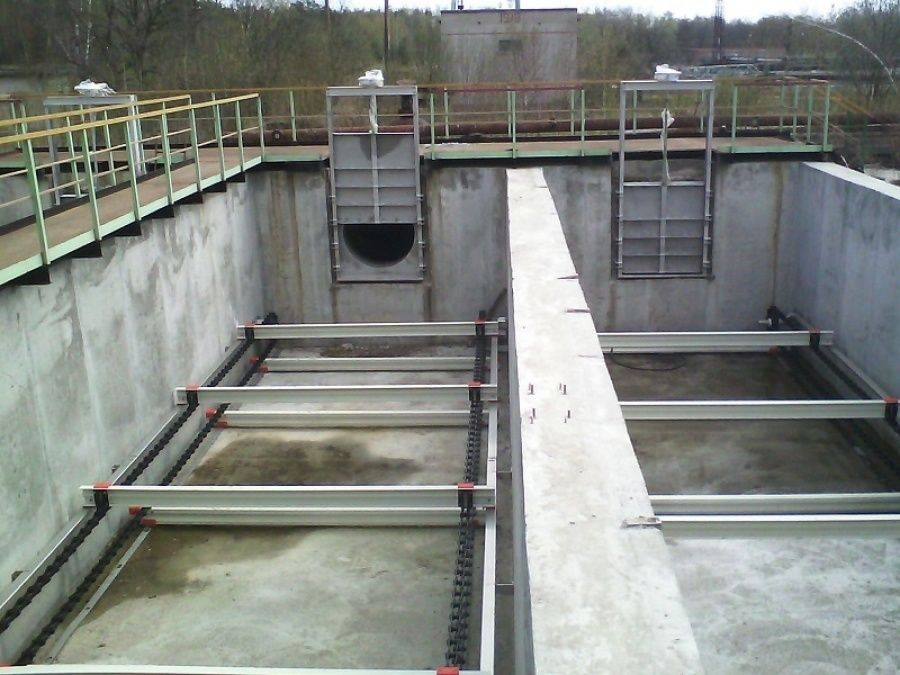
\includegraphics[width=0.8\linewidth]{HorizontalGritChamber}
    \caption{Horizontal grit chamber}
  \end{subfigure}
  \hspace{0.2cm}
  \begin{subfigure}[b]{0.5\linewidth}
    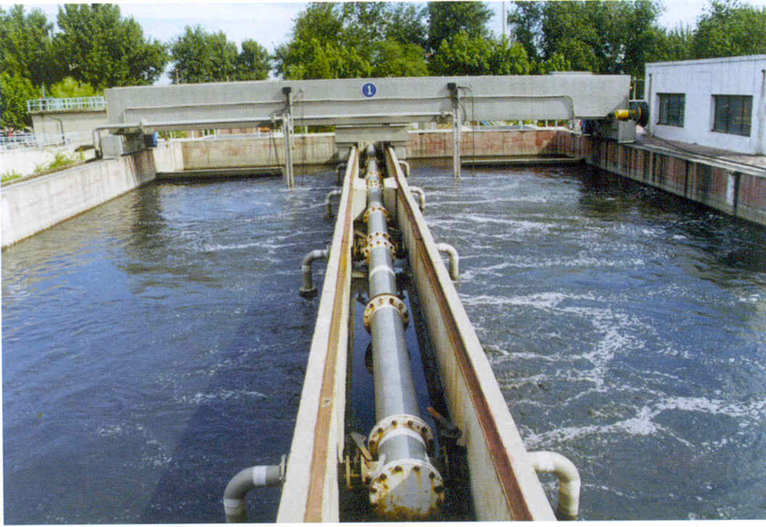
\includegraphics[width=0.8\linewidth]{AeratedGritChamber}
    \caption{Aerated grit chamber}
  \end{subfigure}
\end{figure} 					

\begin{figure}[h!]
  \centering
  \begin{subfigure}[b]{0.47\linewidth}
    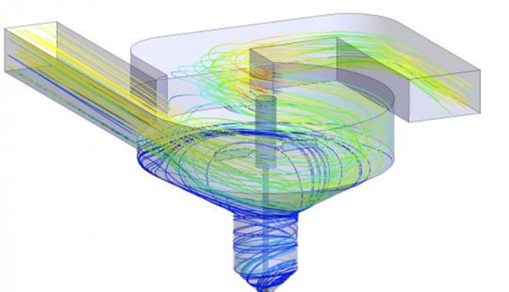
\includegraphics[width=0.8\linewidth]{VortexGritChamber1}
    \caption{Vortex grit chamber design}
  \end{subfigure}
  \hspace{0.2cm}
  \begin{subfigure}[b]{0.43\linewidth}
    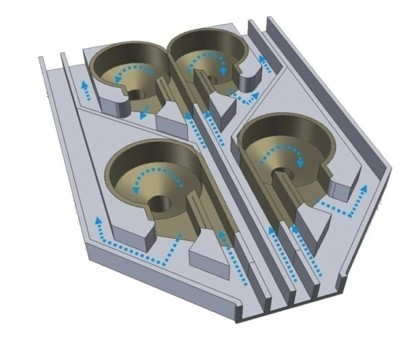
\includegraphics[width=0.8\linewidth]{VortexGritChamber}
    \caption{Vortex grit chamber installed}
  \end{subfigure}
\end{figure} 

\subsection{Pre-aeration}\index{Pre-aeration}	
	\begin{itemize}
		\item Pre-aeration of the wastewater as part of the preliminary treatment may be provided as a separate process or increased detention time in an aerated grit chamber.
		\item Pre-aeration provides the follwoing benefits:
			\begin{itemize}
				\item freshens up wastewater by dissolving oxygen thereby reducing the wastewater septicity
				\item reduction of septicity allows for better settling - solids and BOD removal, in the following primary treatment process
				\item promotes grease separation which facilitates its removal during primary treatment
			\end{itemize}
	\end{itemize}
\subsection{Flow Equalization}\index{Flow Equalization}	

	\begin{itemize}
		\item Flow equalization involves storing a portion of peak flows for release during low-flow periods
		\item It prevents surges and allows for the operation of processes at design flows thus allowing for optimal physical, biological and chemical processes to take place.
		\item It results in saving capital costs as the processes may be built with a treatment capacity which is less than the peak flows
	\end{itemize}
\newpage
\section{Primary Treatment}\index{Primary Treatment}	

\begin{itemize}
\item Synonyms:  primary treatment basin, primary clarifier, sedimentation basin, primaries, clarifier

	
		\item Primary treatment is after preliminary treatment and 				before secondary treatment
		\item Its two main objectives are: 
			\begin{itemize}
				\item Remove settleable solids
				\item Remove floatable solids
			\end{itemize}
		\item This is a physical process which relies on the physical 			properties - how heavy or light the suspended solids particles 		are to effect its separation
		\item Provides quiescent conditions for the influent 					wastewater for the heavier solids to settle and the lighter 			solids to float
		\item Removes settleable solids and floatables
		\item Settled solids are removed as sludge from the bottom of 			the clarifier
		\item Floatable solids including oil and grease are also 				removed, as scum from the surface\\
		\item The shape of the primary clarifier is either rectangular 		or circular
	
		\item Effective solids removal in the primary clarifiers will 			reduce the loading on the expensive secondary treatment 				process.
		\item The amount of solids removed during primary treatment 			may be enhanced by chemical addition - ferric or ferrous 				chloride as a coagulant and anionic polymer as the flocculant.  		This is called Chemically Enhanced Primary Treatment (CEPT).
		\begin{center}
				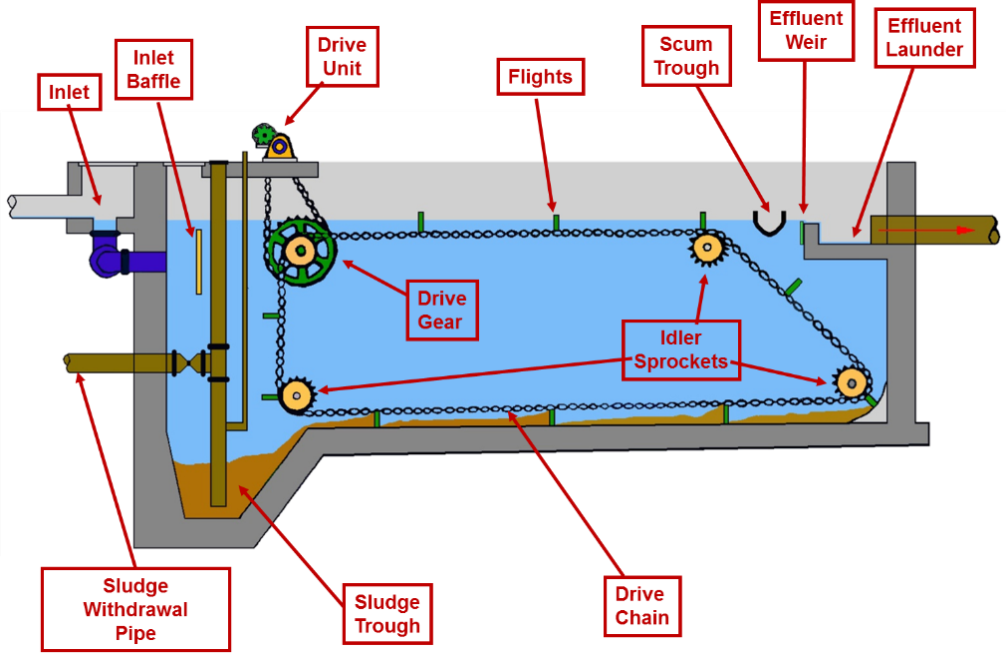
\includegraphics[scale=0.9]{RectangularClarifier}\\
				Cross section of a Rectangular Clarifier\\
				
\includegraphics[scale=0.1]{Blank}\\
				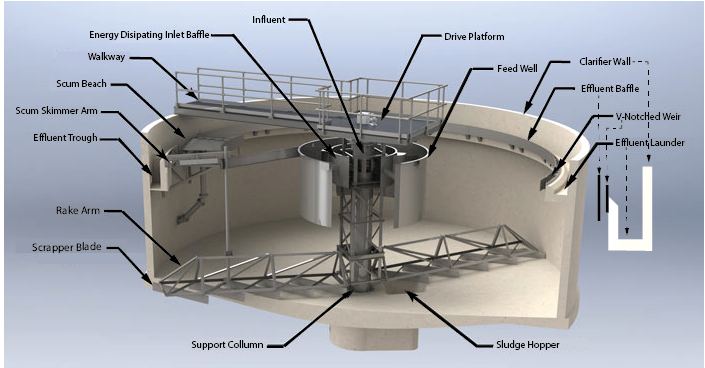
\includegraphics[scale=0.5]{CircularClarifier3}\\
				Cross section of a circular clarifier\\
			\end{center}
				
\includegraphics[scale=0.03]{Blank}\\
\item \textbf{Typical Removal Rates:}\\
\begin{itemize}
\item \hspace{10mm} BOD removal – 25\% to 40\% and about 60\% with CEPT
\item \hspace{10mm} Suspended solids (SS) removal – 40\% to 60\% and about 75\% with CEPT
\item \hspace{10mm} Settleable Solids removal - $>$90\%
\end{itemize}
\end{itemize}

